\section{RQ3: Metadata of Real MCP Servers}

\subsection{Method}

We ran two surveys, each under a protocol confirmed before the sampling frame was built.
\begin{itemize}
  \item \textbf{Sampling.} For each information type, a fixed GitHub query \code{"<keyword> mcp server"} sorted by stars; the result list was locked with SHA-256 before any code was read, with predefined fallback queries for thin categories. Survey~1 covers 7 types (weather, currency exchange, stocks, crypto, geocoding, web search, news) with 6 servers each: 42 servers and 105 pairs. Survey~2 is a new sample that excludes every survey-1 repository, adds 5 types (translation, IP geolocation, movies, books, air quality) and takes 8 servers per type: 78 servers, of which 74 (245 pairs) enter pooled estimates because two types had fewer than 4 eligible servers.
  \item \textbf{Screening} in rank order against five criteria: public repository; a real Model Context Protocol implementation; a tool returning the information type; an external API call; a default upstream. Screening errors found during coding were corrected by the predefined rank-order rule (1 in survey 1, 4 in survey 2).
  \item \textbf{Ground truth.} Static reading of the code at a pinned commit, without running it, to identify the provider each tool calls by default, with \code{file:line} evidence. Two servers \emph{share} if their default provider sets intersect.
  \item \textbf{Declared metadata.} Only providers named explicitly at L1 or L2 count.
  \item \textbf{Data-origin level.} Post hoc in survey 1, \emph{preregistered} in survey 2 using only evidence inside the repositories, in two variants: a literal reading of names, and an informed reading that knows, for example, that Frankfurter distributes ECB data.
  \item \textbf{Predictions.} Six predictions P1--P6 derived from survey 1, each with a pass rule written in advance. Three amendments, each made before the affected metrics were computed: A1 clarified the codebook; A2 recorded five interpretation rules that arose during coding and the analysis implementation; A3 defined the author-adjudication procedure.
  \item \textbf{Coding.} Coder A is an AI (Claude). A second coder (a team member) independently coded 10 servers in survey 1 and 20 in survey 2, chosen by hash, but \emph{used an AI (Claude or Codex)}, contrary to the plan of a human coder. Agreement is therefore between AI coders.
\end{itemize}

\subsection{Results}

\paragraph{Survey 1} (operator level). $\rho = 17/105 = 0.16$ (server-level bootstrap 95\% CI $[0.075,0.281]$), highest for web search (0.47). L1 metadata is missing in \textbf{70\%} of pairs; where present, $r=8/8$ and $\varphi=0/24$. At L2, $m=0.05$, $r=17/17$, $\varphi=0/83$. At the data-origin level (post hoc), literal-name recall drops to 0.61 (17/28), and every web-search pair shares at least one engine.

\paragraph{Survey 2} (operator level). $\rho = 67/245 = 0.27$ $[0.179,0.374]$. $\rho$ varies widely by type: currency 0.64 (six servers use Frankfurter), web search 0.39, weather 0.36, down to translation 0.04. L1 metadata is missing in \textbf{71\%} of pairs, and in every pair for weather and stocks; where present, $r=23/27$, $\varphi=3/45$, $J=0.79$. At L2, $m=0.22$, $r=52/55$, $\varphi=7/135$, $J=0.89$ (\cref{tab:origin}).

\begin{table}[t]
\centering
\caption{Survey 2 at the operator and data-origin levels (L2 metadata).}
\label{tab:origin}
\begin{tabular}{lrllr}
\toprule
Level & $\rho$ & $r$ & $\varphi$ & $J$ \\
\midrule
Operator & 0.27 & 0.95 (52/55) & 0.05 (7/135) & 0.89 \\
Data origin, literal names & 0.31 & 0.83 (55/66) & 0.03 (4/124) & 0.80 \\
Data origin, informed & 0.31 & 0.97 (64/66) & 0.02 (2/124) & 0.95 \\
\bottomrule
\end{tabular}
\end{table}

\Cref{tab:pred} checks the preregistered predictions. Two survey-1 findings do \emph{not} replicate: that labels are never wrong when present, and that web search has no independent source. All three L1 false-sharing pairs arise because metadata names the \emph{data source behind} the API rather than its operator; for example, a server calls the Blockchain Academics API while its description says prices come ``via CoinGecko''. At the data-origin level two of these three labels are correct. This interpretation is post hoc; the primary result for P3 remains a failure.

\begin{table}[t]
\centering
\caption{Preregistered predictions of survey 2.}
\label{tab:pred}
\small
\begin{tabular}{p{5.6cm}p{3.6cm}p{4.2cm}}
\toprule
Prediction & Rule & Result \\
\midrule
P1 Sharing exists but is not common & $0.05 \le \rho \le 0.30$ & 0.27, \textbf{met} (CI upper bound 0.37) \\
P2 L1 labels are usually missing & $m_{L1} > 0.50$ & 0.71, \textbf{met} \\
P3 Present labels are rarely wrong & $\varphi_{L1} \le 0.05$ & 0.067 (3/45), \textbf{not met} \\
P4 Operator names miss origin-level dependence & $r_{\text{origin}} < r_{\text{operator}}$ (L2) & 0.83 $<$ 0.95, \textbf{met} \\
P5 Some type has no independent source & $\rho_{\text{origin}} \ge 0.80$ for some type & max 0.71 (web search), \textbf{not met} \\
P6 Real metadata has $J>0$ & $J_{\text{operator},L2} > 0$ & 0.89, \textbf{met} \\
\bottomrule
\end{tabular}
\end{table}

\begin{figure}[t]
  \centering
  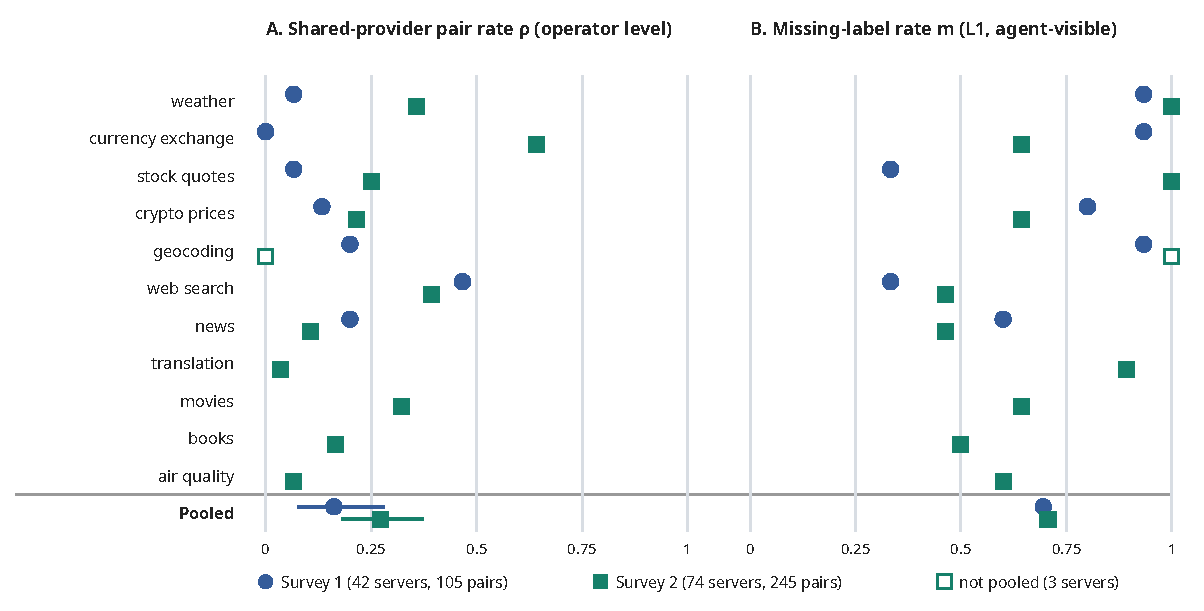
\includegraphics[width=\linewidth]{figures/rq3-surveys.pdf}
  \caption{(A) Operator-level shared-provider rate $\rho$ and (B) L1 missing-label rate $m$, by information type, for survey 1 (circles) and survey 2 (squares). The pooled row shows the 95\% bootstrap interval for $\rho$. $\rho$ for the same type changes sharply between samples, while pooled $m$ is almost unchanged (0.70 and 0.71).}
  \label{fig:surveys}
\end{figure}

\paragraph{Projection onto the selector model} (not a measurement of agents). With the label rates observed in survey 2, the probability of choosing a shared corroborator is 0.436 for random selection, 0.289 with L1 metadata, and 0.109 if README-level information were present in tool descriptions.

\subsection{Label Reliability}

\paragraph{Agreement between AI coders.} In survey 1, after name normalisation, agreement is 0.80 on upstream providers (Cohen's $\kappa=0.78$) and 1.00 on L1. In survey 2 (Claude versus Codex), with a name table fixed in advance, agreement is 0.45 on upstream ($\kappa=0.43$) and 0.65 on L1 ($\kappa=0.57$). Most disagreements are different names for the same organisation (e.g.\ \code{Google Maps Platform} versus \code{Google}); after post-hoc organisation-level merging, agreement is 0.85 on upstream and 0.80 on L1. Most importantly, whether an L1 label is present, the quantity behind the main finding, agrees on \textbf{20/20} servers ($\kappa=1.00$).

\paragraph{Author adjudication.} Lacking a human coder, the author followed a procedure recorded in the protocol before seeing the cases: he chose four codebook rules where the two AI coders diverged (e.g.\ ``the provider is the ultimate data source'' and ``providers not enabled by default do not count''), adjudicated four cases with blinded answers, and checked 10 randomly sampled \code{file:line} evidence citations, all of which were correct. Applying these rules to all 78 servers changes 7 labels. P1, P2, P4, P5 and P6 are unchanged; P3 moves from 3/45 to 2/45 $=0.044$. The false-sharing rate therefore sits \emph{at the 5\% threshold} and depends on the definition. This adjudication is not independent: the author agreed with coder A in 7 of 8 decisions, coder A also explained the questions, and the author read code lines quoted by coder A.
